% sample.tex
\documentclass[pdf,swa,slideBW,nocolorBG,nototal]{prosper}
%\usepackage{ngerman}
\usepackage{graphicx}
\usepackage{wrapfig, rotating}
\usepackage[T1]{fontenc}

\title{Tracing Object Lifetime}
\author{Christoph Neijenhuis, Tobias Mohr, Tim Felgentreff}
%\email{\{christoph.neijenhuis, tobias.mohr, fim.felgentreff\}@student.hpi.uni-potsdam.de}
\institution{
        Agile Software Development \\
        Hasso-Plattner-Institut \\
        Universit�t Potsdam\\
        SS 2011
}
\foot{Agile Software Development 2011 | Felgentreff, Mohr, Neijenhuis | \today }

\begin{document}

\maketitle

\begin{slide}{Demo}
  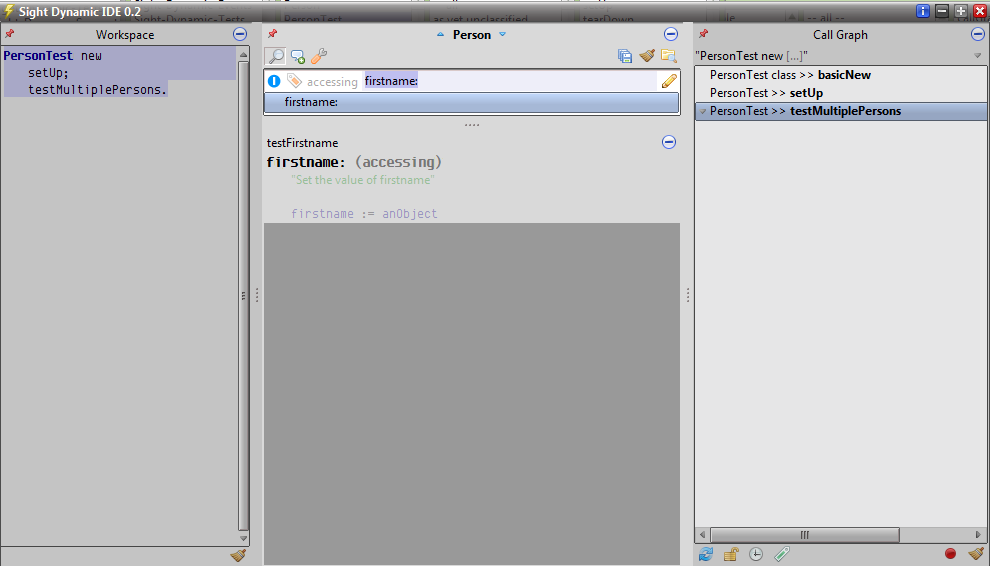
\includegraphics[width=\linewidth]{pics/sdide_intro}
\end{slide}

\overlays{2}{%
\begin{slide}{Demo}
  \begin{itemize}
  \item During its lifetime an object is \ldots
    \begin{itemize}
    \item created from a class,
    \item referenced in different contexts,
    \item called upon,
    \item and modified.
    \end{itemize}
  \end{itemize}
  \fromSlide{2}{%
  \begin{itemize}
    \item The call graph tracer is a way to ask questions
    \begin{itemize}
    \item Where did this object come from?
    \item Who calls it and when?
    \item Where and how is it modified?
    \item How does it arrive at a particular point?
    \end{itemize}
  \end{itemize}}
\end{slide}}

\begin{slide}{Agenda}
  \begin{itemize}
  \item Infrastructure
  \item Planning
  \item User stories
  \item Tests
  \end{itemize}
\end{slide}

\begin{slide}{Infrastructure}
  \parbox[t]{0.6\textwidth}{%
    \vspace*{2.5cm}
    \hspace*{5cm}
    \begin{rotate}{0}
      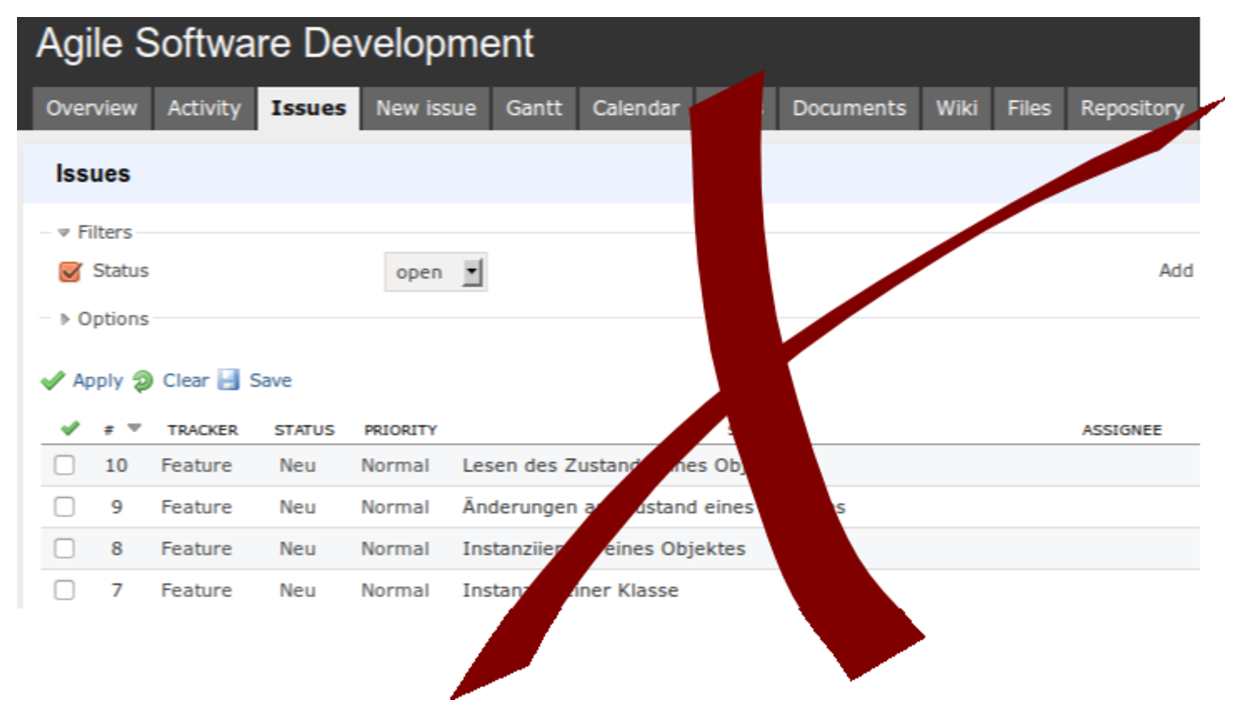
\includegraphics[width=\linewidth]{pics/redmine}
    \end{rotate}}
  \parbox[t]{0.6\textwidth}{%
    \vspace*{5cm}
    \hspace*{4cm}
    \begin{rotate}{0}
      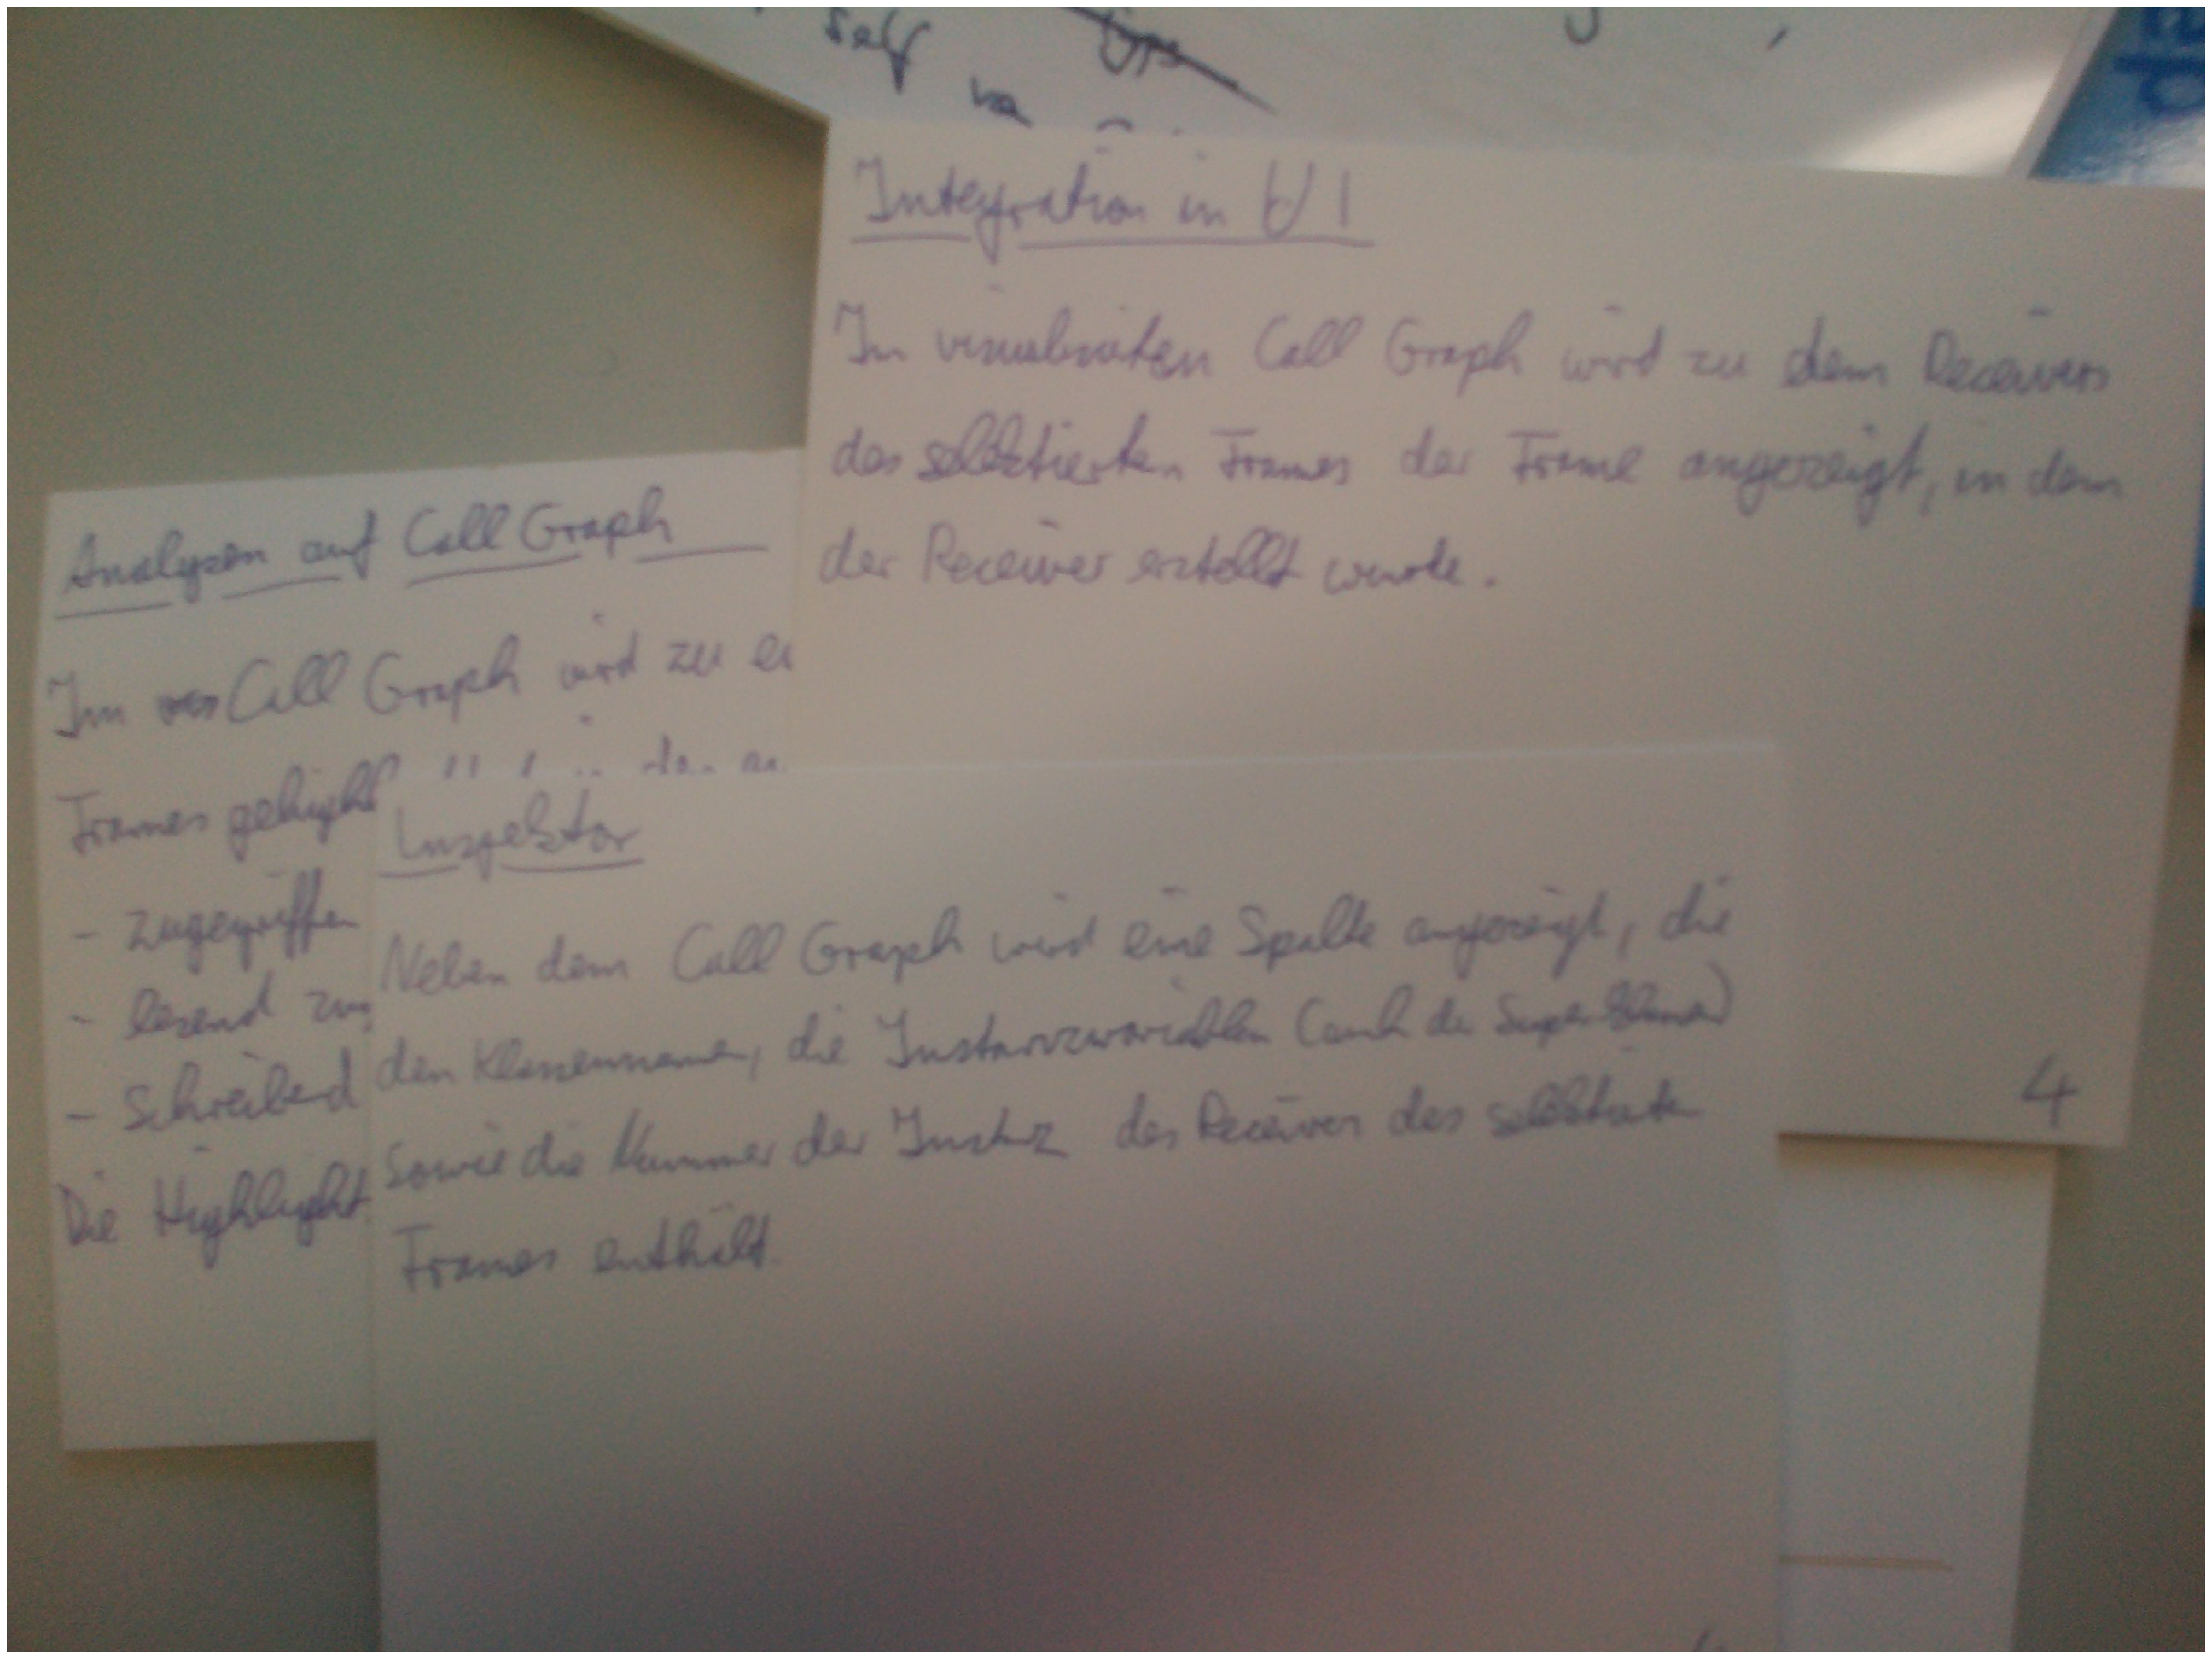
\includegraphics[width=\linewidth]{pics/user_stories}
    \end{rotate}}
  \vspace*{-8cm}
  \begin{itemize}
  \item {\it Full-blown ticket system} ~\\~\\~\\~\\~\\
  \item {\bf Story cards}
  \end{itemize}
\end{slide}

\begin{slide}{Planning}
  \begin{itemize}
  \item Initial meeting with customer and developer of base system
    \begin{itemize}
    \item Extensive overview about problem space
      \begin{itemize}
      \item Underestimated the meeting time, taking more notes would have
        been useful
      \end{itemize}
    \item Introduction into new IDE
    \end{itemize}
  \item Bi-weekly customer meetings
  \end{itemize}
\end{slide}

\begin{slide}{User Stories}
  \parbox[t]{0.6\textwidth}{%
    \vspace*{3.5cm}
    \hspace*{5cm}
    \begin{rotate}{353}
      
\includegraphics[width=\linewidth]{pics/user_story}
    \end{rotate}}
  \vspace*{-2.5cm}
  \begin{itemize}
  \item Written during customer meetings
  \item Titled for quick reference
  \item Valued immediately afterwards
  \item Commitment for next sprint determined in a quick follow-up meeting
  \end{itemize}
\end{slide}

\begin{slide}{Tracing our stories}
  \begin{centering}
    \includegraphics[width=\linewidth]{pics/bad_trace_1}
  \end{centering}
  \raggedleft{Not as ``direct'' and ``clean'' as we would like}
\end{slide}

\begin{slide}{Tracing our stories}
  \hskip-1em
  \includegraphics[width=1.1\linewidth]{pics/bad_trace_2}
\end{slide}

\begin{slide}{Problems with our stories}
  \begin{itemize}
  \item User-stories are reflected in test names, but not in test
    code (much)
  \item Tests aren't written before implementing the story
  \item Estimated time and required time isn't tracked per story
  \end{itemize}
\end{slide}

\overlays{4}{%
\begin{slide}{Tests}
  \begin{itemize}
  \item Tests were developed in parallel to the implementation
    \fromSlide{2}{%
      \begin{itemize}
      \item As a quicker workspace
      \item To run examples quickly
      \fromSlide{3}{%
      \item \ldots, but not to test user stories}
    \end{itemize}}
  \fromSlide{4}{%
  \item $\Rightarrow$ It's hard to write tests in the beginning}
  \end{itemize}
\end{slide}}

\begin{slide}{Tests}
  \begin{minipage}{0.6\linewidth}
    \begin{centering}
      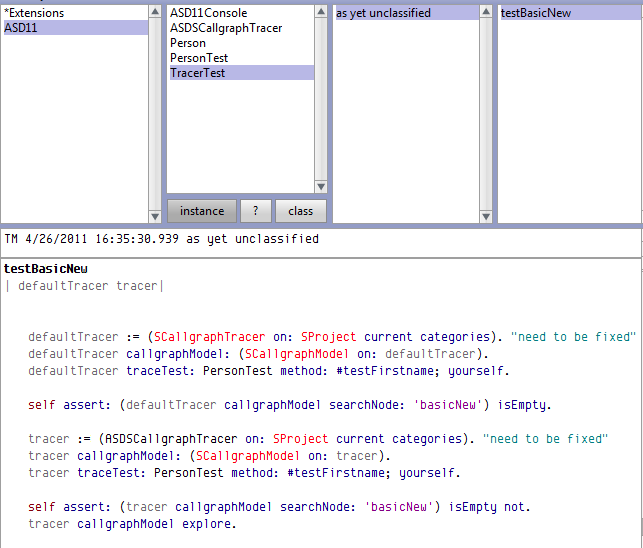
\includegraphics[width=\linewidth]{pics/workspace_test}
    \end{centering}
  \end{minipage}
  \begin{minipage}{0.3\linewidth}
    \raggedright{Note the {\bf \#explore} at the bottom}
  \end{minipage}
\end{slide}

\overlays{3}{%
\begin{slide}{Problems with testing}
  \begin{itemize}
  \item Criticism from the customer after first sprint
  \fromSlide{2}{%
    \begin{itemize}
    \item Tests are hard to understand
    \item Tests are not easily matched to user stories
    \end{itemize}
  }
  \end{itemize}
  \fromSlide{3}{%
    \raggedleft{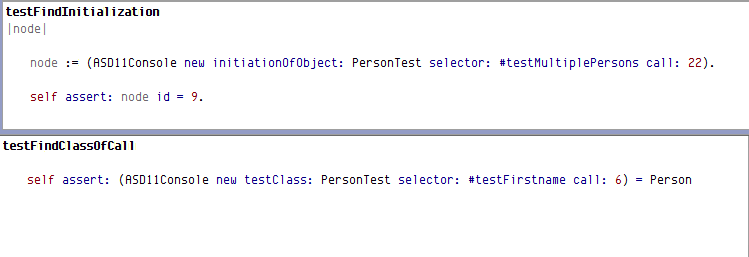
\includegraphics[width=0.8\linewidth]{pics/bad_tests}}
  }
\end{slide}}

\overlays{2}{%
\begin{slide}{Problems with testing}
  \begin{itemize}
  \item For the second sprint we started with implementing the tests
    first, \ldots
    \begin{itemize}
    \item \ldots but then decided to re-implement based on different code.
    \end{itemize}
  \fromSlide{2}{%
  \item At the end of Sprint \#2, we don't have tests for all functionality}
  \end{itemize}
\end{slide}}

\begin{slide}{Conclusions}
  \begin{itemize}
  \item We're doing well estimating overall time
    \begin{itemize}
    \item The first sprint we managed to implement all, the second
      half the stories
    \item Our estimates were off on the work required to acquaint
      ourselves with the framework
    \item Tickets, as well as stories, would be nice to track that
      ``additional work''
    \end{itemize}
  \item We need to track our time per story more closely to get better
    on that granularity, too
  \item We have to be more stringent with {\bf ``test first''}
  \item We need tests to begin with
  \end{itemize}
\end{slide}

\begin{slide}{}
  \nocite{*}
  \bibliographystyle{splncs}
  {\small \bibliography{swt.bib}}
\end{slide}

\end{document}
